%%%%%%%%%%%%%%%%%%%%%%%%%%%%%%%%%%%%%%%%%%%%%%%%%%%%%%%%%%%%%%%%%%%%%%%%%%%%%%%%
%2345678901234567890123456789012345678901234567890123456789012345678901234567890
%        1         2         3         4         5         6         7         8

\documentclass[letterpaper, 10 pt, conference]{ieeeconf}  % Comment this line out
                                                          % if you need a4paper
%\documentclass[a4paper, 10pt, conference]{ieeeconf}      % Use this line for a4
                                                          % paper

\IEEEoverridecommandlockouts                              % This command is only
                                                          % needed if you want to
                                                          % use the \thanks command
\overrideIEEEmargins
% See the \addtolength command later in the file to balance the column lengths
% on the last page of the document



% The following packages can be found on http:\\www.ctan.org
\usepackage{graphicx} % for pdf, bitmapped graphics files
%\usepackage{epsfig} % for postscript graphics files
%\usepackage{mathptmx} % assumes new font selection scheme installed
%\usepackage{times} % assumes new font selection scheme installed
%\usepackage{amsmath} % assumes amsmath package installed
%\usepackage{amssymb}  % assumes amsmath package installed
\usepackage{epstopdf}
\usepackage{siunitx}
\usepackage{hyperref}
\usepackage{lineno}
\linenumbers

\title{\LARGE \bf
Modeling and simulation of the R5912 photomultiplier for the LAGO project
}

\author{S. Hern\'andez-Barajas$^{1}$, Y. Le\'on-Carre\~no$^{1}$, J. Pe\~na-Rodr\'iguez$^{2}$, L. A. N\'u\~nez$^{2,3}$\\ for the LAGO collaboration$^{4}$% <-this % stops a space
\thanks{$^{1}$ Escuela de Ingenierías El\'ectrica, Electr\'onica y de Telecomunicaciones, Universidad Industrial de Santander, Carrera 27 y Calle 9, 640002 Bucaramanga, Colombia.
}
\thanks{$^{2}$Escuela de F\'isica, Universidad Industrial de Santander, Carrera 27 y Calle 9, 640002 Bucaramanga, Colombia.}
\thanks{$^{3}$Centro de F\'isica Fundamental, Departamento de F\'isica, Universidad de Los Andes, 5101 M\'erida, Venezuela.}
\thanks{$^{4}$The complete author list and institutions at \url{http://lagoproject.net/collab.html}}
}


\begin{document}
\maketitle
\thispagestyle{empty}
\pagestyle{empty}

% , A. V\'asquez-Ram\'irez$^{2}$


%%%%%%%%%%%%%%%%%%%%%%%%%%%%%%%%%%%%%%%%%%%%%%%%%%%%%%%%%%%%%%%%%%%%%%%%%%%%%%%%
\begin{abstract}
We present the results of modeling and simulating the Hamamatsu R5912 photomultiplier tube that is used in most of the sites of the LAGO collaboration. The model was compared with data of in-operation water Cherenkov detectors (WCD) installed at Bucaramanga-Colombia and Bariloche-Argentina. The LAGO project is an international experiment that spans across Latin America at different altitudes joining more than 35 institutions of 11 countries. It is mainly oriented to basic research on gamma-ray bursts and space weather phenomena. The LAGO network consists of single or small arrays of WCDs composed mainly by a photomultiplier tube and a readout electronics that acquires single-particle or extensive air shower (EAS) events triggered by the interaction of cosmic rays with the Earth atmosphere. 
\end{abstract}

%%%%%%%%%%%%%%%%%%%%%%%%%%%%%%%%%%%%%%%%%%%%%%%%%%%%%%%%%%%%%%%%%%%%%%%%%%%%%%%%

\section{INTRODUCTION}

Astrophysical phenomena are studied by means of giant cosmic ray (CR) observatories spread around the world. Such experiments, located at ground level, detects atmospheric particle showers resulting from the interaction of high energy primary CRs with atmospheric gases. The EAS detection is made using different techniques, taking advantage of the signal that charged particles leave along their pathway. At ground level the EAS is detected by arrays of Cherenkov counters, scintillators or antennas getting information of the shower front, composition and primary energy \cite{Bertou2006, Galindo2017}. The longitudinal development of the EAS is directly interpreted from the electromagnetic radiation created by photons, electrons and positrons crossing the atmosphere. This EAS component is detected by fluorescence telescopes \cite{Neesal2011}, Imaging Atmospheric (or Air) Cherenkov Telescopes (IACTs) \cite{Schoorlemmer2019} and radio antennas \cite{Aab2016, Schrder2016}.

The LAGO project was founded with the goal of creating a collaborative project in astroparticle physics research to train young scientists in Latin America. LAGO consists of a network of own made water Cherenkov detectors (WCD) spanning over different sites, located at several latitudes (from Mexico to the Antarctic) and altitudes (from sea level up to 5000 m a.s.l.) \cite{Sidelnik2016}. 

The WCD network of LAGO is able to detect short duration transients --like gamma-ray bursts (GRBs)-- and long duration transients --like Forbush decreases-- \cite{Durn2016,Asorey2018} by searching changes in the cosmic ray background recorded using the single particle technique \cite{Vernetto2000, Leon2018}. LAGO operates in energies ranging from 0.5 GeV to tens of TeV.

LAGO detectors are made up of cylindrical containers of plastic, metal or fibreglass with an internal Tyvek coating for enhancing its optical properties (reflection and diffusion) and the transmission efficiency of Cherenkov photons generated by crossing charged particles. The Cherenkov radiation is usually collected by an 8$^{\prime\prime}$ Hamamatsu R5912 photomultiplier tube (PMT) located at the center of the WCD cover. The pulses generated by the anode and last dynode of the PMT are digitized by a 10-bit fast analog-to-digital converter (FADC) working at 40\,MHz. A 12-sample records the pulses with a 25 ns resolution timestamp.

A key point in the LAGO WCDs is the calibration process. We establish a conversion rule from the digitized charge in electronic units to deposited energy in vertical-equivalent muons (VEM) \cite{Bertou2006, Galindo2017}. This relationship depends on the linearity of both the PMT and the readout electronics, working together. 

This paper propose a general PMT and bias chain model which is tuned with the LAGO's current PMT parameters. The model allow us to assess the electronics front-end linearity under different acquisition conditions. The SPICE simulation performance is validated with data measurements from the Nahuelito, Chitaga, and MuTe detectors. 

\section{METHODS}

\subsection{A generic PMT model}

\begin{figure}[h!]
\begin{center}
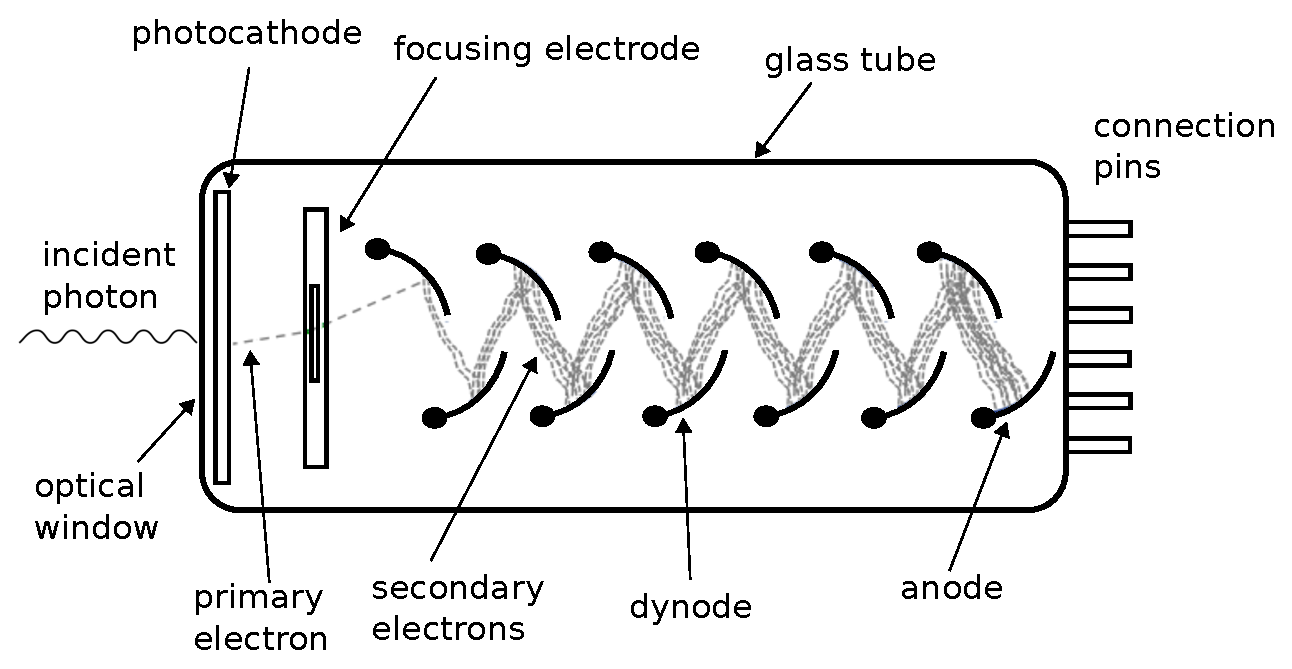
\includegraphics[width=0.48\textwidth]{Figures/PMT.eps}
\caption{PMT functioning sketch. The incident photon impinges the photocathode releasing a primary electron which create a secondary electron avalanche due to the electric field generated along the dynodes. All the PMT parts are encapsulated in a vacuum glass tube.}
\label{PMT_sketch}
\end{center}
\end{figure}

A PMT is an optoelectronic device which generates a measurable electric current ($\sim$ mA) by means of the photoelectric effect when a photon impinges its photocathode. The photoelectron is accelerated by a potential difference reaching the energy for pulling up more electrons from the next dynode. This avalanche of secondary electrons along the dynodes amplifies the anode current with gain factors of $\sim10^6$-$10^7$. (See Fig. \ref{PMT_sketch}).

We modeled the PMT R5912 taking into account such basic principle of functioning and its intrinsic parameters: the number of amplification stages and the gain curve. The total gain of the PMT model is defined as:

\begin{equation}
G = \frac{I_a}{I_k}
\end{equation}

\noindent where $I_a$ is the anode current and $I_k$ is the photocathode current.

The PMT gain can be expressed as a function of the gain in each stage,

\begin{equation}
G =  \beta \prod_{i=1}^{N}  g_i 
\end{equation}

\noindent where $g_i$ is the gain in each stage, $N$ is the number of dynodes and $\beta$ is the collection efficiency. The gain $g_i$ depends on the inter-dynode voltage $v_i$,
%If $ \eta \approx 100\%$, then

\begin{equation}
g_i = k_i v_i^\alpha
\end{equation}

\noindent where $k_i$ is a constant and $ 0.6  \leq \alpha \leq 0.8$ is an intrinsic parameter of the PMT. The total gain (2) can be expressed as the product of all the inter-dynode gains or in function of the PMT bias voltage $V_B$,

\begin{equation}
G =  \prod_{i=1}^{N}  k_i (V_B \epsilon_i)^{\alpha} 
\label{eq::gain}
\end{equation}
where $\epsilon_i$ is the fraction of the bias voltage in each inter-dynode stage as a result of the resistor polarization chain.

The fraction of the bias voltage is defined as 

\begin{equation}
\epsilon_i = \frac{R_i}{R_T}
\end{equation}

where $R_i$ is the interdynode resistance and $R_T$ is the total resistance of the polarization chain.

To simplify the model, we can assume that $k_i$ values are equal for all dynodes due it depends on the dynode material \cite{Akimov2017}. Equation \ref{eq::gain} is transformed in

\begin{equation}
G =  k^N V_B^{N\alpha} \left ( \prod_{i=1}^{N} \epsilon_i \right)^{\alpha} 
\label{eq::gainkte}
\end{equation}

We define $\varepsilon$, to estimate the value of $\alpha$ and $k$, as

\begin{equation}
    \varepsilon = \sqrt[N]{\prod_{i=1}^{N} \epsilon_i}
    \label{eq::varep}
\end{equation}
Using the equation \ref{eq::varep} in \ref{eq::gainkte}, the gain is expressed as follows,

\begin{equation}
G = k^N (V_B \varepsilon)^{N\alpha}  
\label{eq::gainmodel}
\end{equation}

\subsection{Modeling the PMT R5912}

\begin{figure}[h!]
\begin{center}
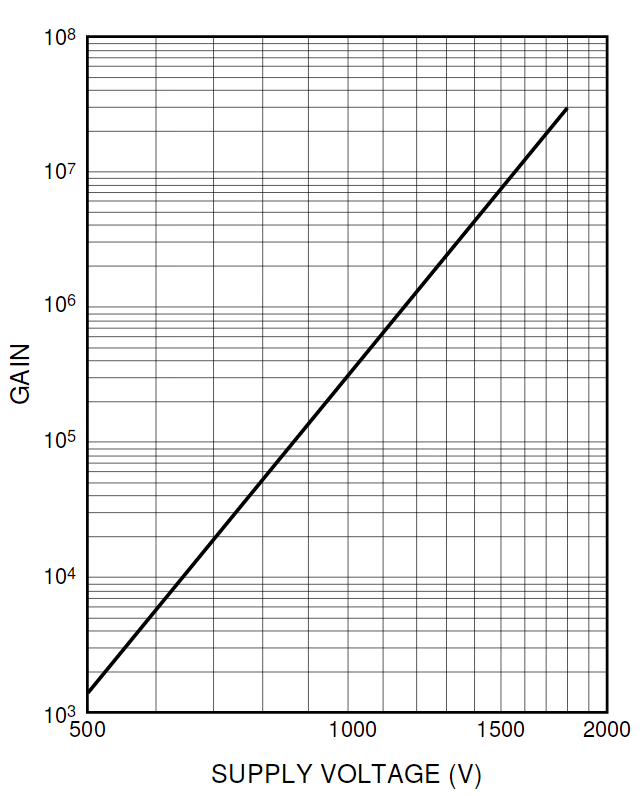
\includegraphics[width=0.4\textwidth]{Figures/Gain_curve}
\caption{Gain curve of the PMT R5912.The gain of the PMT has an exponential relation depending on the high voltage applied between the anode and cathode \cite{Hamamatsu2019}.}
\label{Gain_curve}
\end{center}
\end{figure}

To get the parameters $\alpha$ and $k$, a couple of points $[V_{B1}, G_1]$ and $[V_{B2}, G_2]$ are extracted from the gain curve of the PMT Hamamatsu R5912 \cite{Hamamatsu2019}. (See Fig. \ref{Gain_curve}).

The values $[1000 V, 3 \times 10^5 ]$ and $[1500 V, 7 \times 10^6]$ were chosen. We derived a pair of equations from (5) with the given points to solve the unknown variables ($\alpha$, $k$).

\begin{equation}
G_{1} = k^N (V_{B1} \varepsilon)^{N \alpha}
\label{eq:gain1}
\end{equation}

\begin{equation}
G_{2} = k^N (V_{B2} \varepsilon)^{N \alpha}
\label{eq:gain2}
\end{equation}

\noindent where the number of dynodes is $N=10$. The parameter $\varepsilon$ is calculated by means of the voltage distribution ratio in the resistive polarization chain, provided in the PMT datasheet, as shown in Table \ref{net}.

\begin{equation}
\varepsilon = 0.035
\end{equation}

\begin{table}[ht]
\centering
  \caption{Tapered voltage distribution of the PMT R5912 for linear measurements \cite{Hamamatsu2019}.}
  \begin{tabular}{ | c | c | c |}
    \hline
    Electrodes & $R_i$ & $\epsilon_i$ \\ \hline
    K-Dy1 & 11.3 & 0.308 \\ \hline
    Dy1-F2 & 0 & 0 \\ \hline
    F2-F1 &  0.6 & 0.016 \\ \hline
    F1-F3 & 0 & 0 \\ \hline
    F3-Dy2 & 3.4 & 0.092 \\ \hline
    Dy2-Dy3 & 5 & 0.136 \\ \hline
    Dy3-Dy4 & 3.33 & 0.090 \\ \hline
    Dy4-Dy5 & 1.67 & 0.045 \\ \hline
    Dy5-Dy6 & 1 & 0.027 \\ \hline
    Dy6-Dy7 & 1.2 & 0.032 \\ \hline
    Dy7-Dy8 & 1.5 & 0.040 \\ \hline
    Dy8-Dy9 & 2.2 & 0.060 \\ \hline
    Dy9-Dy10 & 3 & 0.081 \\ \hline
    Dy10-P & 2.4 & 0.065 \\
    \hline
  \end{tabular}
  \label{net}
\end{table}

% In this case, a linear behavior of the PMT is desired, for this reason, the tapered voltage distribution was chosen. The condition for determining the $\epsilon$ value is
% \begin{equation}
% \epsilon  \sum_i R_i = 1
% \end{equation}
% where $R_i$ is the ratio in each inter-electrode stage $i$. The estimated $\epsilon$ value was 0.02732.

Then, an expression for $k$ is obtained from (\ref{eq:gain2}) as follows,

\begin{equation}
k=\sqrt[N]{\frac{G_2}{(V_{B2}\varepsilon)^{N \alpha}}}
\label{eq:k0}
\end{equation}
\noindent and replacing (\ref{eq:k0}) in (\ref{eq:gain1}) the parameter $\alpha$ is,

\begin{equation}
\alpha=\frac{\log \left( \frac{G_1}{G_2} \right)}{N \log \left( \frac{V_{B1}}{V_{B2}} \right)}
\label{eq:alpha}
\end{equation}
From (\ref{eq:k0}) and (\ref{eq:alpha}) we obtain $k=0.223$ and $\alpha= 0.776$.

\subsection{PMT and passive biasing network Spice simulation}

The dynodes and anode currents were modeled as function of the parameters $k$, $\alpha$ , $\epsilon_i$, $V_B$ and $N$. The current flowing through $i$th dynode is defined as,

\begin{equation}
I_{d,i} = I_k \frac{(k V_B^\alpha)^N \left ( \prod_{i=1}^{N} \epsilon_i \right)^{\alpha}}{(k v_i^\alpha)^{N+1-i} \left ( \prod_{i=1}^{N+1-i} \epsilon_i \right)^{\alpha} }, \ \ \ i=1,2, \cdots N
\label{Id}
\end{equation}

The anode current is:
\begin{equation}
I_a = I_k k^N (V_B \varepsilon)^{N \alpha}
\label{Ia}
\end{equation}

The PMT and the biasing network were simulated using the Orcad Pspice software. We used the GVALUE block to model the PMT currents flowing from the cathode to the anode along each PMT dynode \cite{Krihely2014}. This block sets the transfer function described by the equations \ref{Id} and \ref{Ia} for each amplification stage depending on the voltage applied between adjacent dynodes. 

% \begin{figure}[h!]
% \begin{center}
% 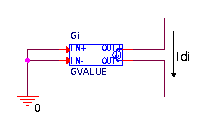
\includegraphics[width=0.35\textwidth]{Figures/GVALUE}
% \caption{Gain block used to simulate the inter-dynode stages.}
% \label{Gval}
% \end{center}
% \end{figure}

Resistive divider networks are the most widely used method to bias PMTs \cite{Camin1999PassiveAA}. We selected a tapered resistive chain with decoupling capacitors to reduce nonlinearities in the PMT response due to space-charge effect (large current flowing in the dynodes) \cite{Huang_2013, Hamamatsu2007}. The resistor values were estimated taking into account the interdynode ratios presented in the Table \ref{net}. Decoupling capacitors of 20 nF were connected (serial and parallel) in the last six dynodes and the anode.

The PMT output signal has a high direct current (DC) bias which can destroy the frontend electronics. We install coupling capacitors of 4.7~nF (C18 and C21) to filter the DC component in the anode and the last dynode output. For avoiding oscillations in the signal due to reflections for bad impedance coupling in the transmission lines we implemented 50 $\Omega$ output loads. 

An amplification stage was connected to the last dynode output to increase the dynamic response/range if the dynode pulse amplitude saturates the readout system we can recover the pulse shape from the anode output. The operational amplifier AD8011 amplifies 20 times the dynode output and inverts its polarity. The Fig. \ref{Circuit} shows the schema of the designed Spice model.

%When the ADC connected to the amplified dynode is saturated because the pulse amplitude exceeds its range, we read the anode output searching for a complete shaped pulse from which we can obtain clean information.

\begin{figure}[h!]
\begin{center}
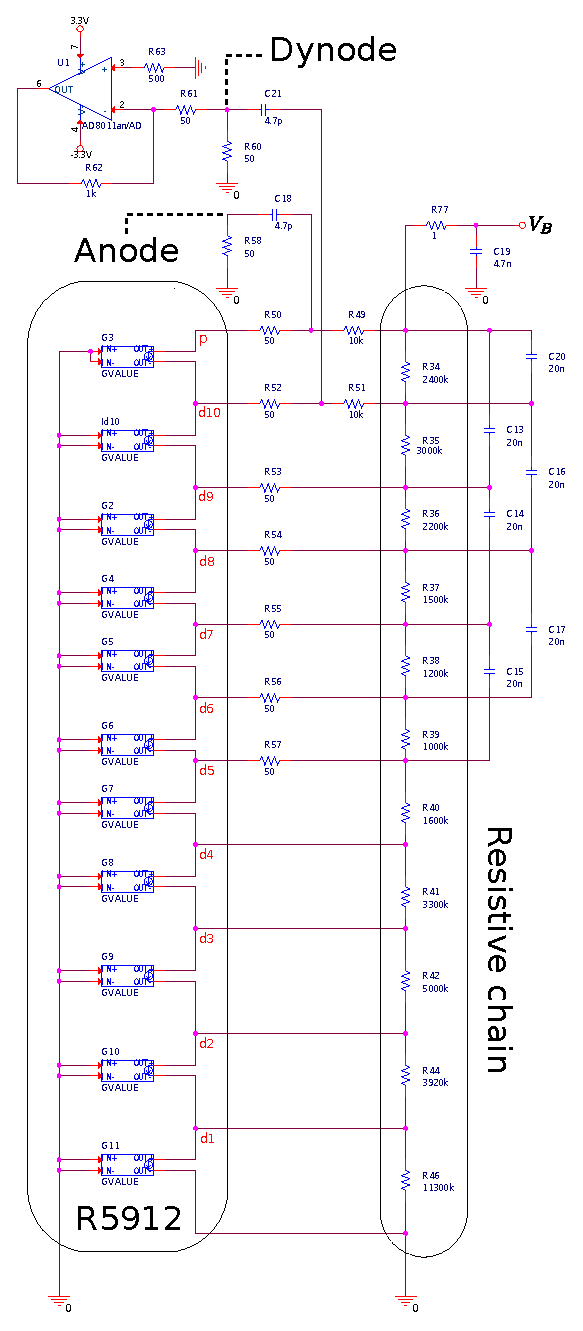
\includegraphics[width=0.45\textwidth]{Figures/Circuit}
\caption{Spice model for the PMT R5912 and the tapered resistive chain.}
\label{Circuit}
\end{center}
\end{figure}

\subsection{Incident photon yield and cathode current}

We carried out simulations using the particle-matter interaction code GEANT4 to characterize the incident photon signal on the PMT cathode generated by charged particles crossing the WCD. We injected 10$^5$ muons of 3 GeV perpendicularly to a 120 cm height WCD \cite{Vasquez2019, Caldern2015}. The average number of Cherenkov photons ($N_{\gamma}$) along the path were 46857, 1617 of such photons reach the PMT optical window and the PMT photocathode releases around 203 photo-electrons ($N_{pe} = \eta N_{\gamma}$) taking into account the maximum quantum efficiency ($\eta = 22 \%$ at 390 nm). 

% The number of photo-electrons is

% \begin{equation}
% N_{pe} = \eta N_{\gamma}
% \end{equation}

The shape of the photoelectron pulse at the PMT photocathode depends on the arrival time of the incident photons as shown in Fig. \ref{pulse_G4}. The pulse decreases exponentially having an time constant of $\sim$42.12~ns and a time width (at the 10$\%$ amplitude) of $\sim$100~ns.\\

\begin{figure}[h!]
\begin{center}
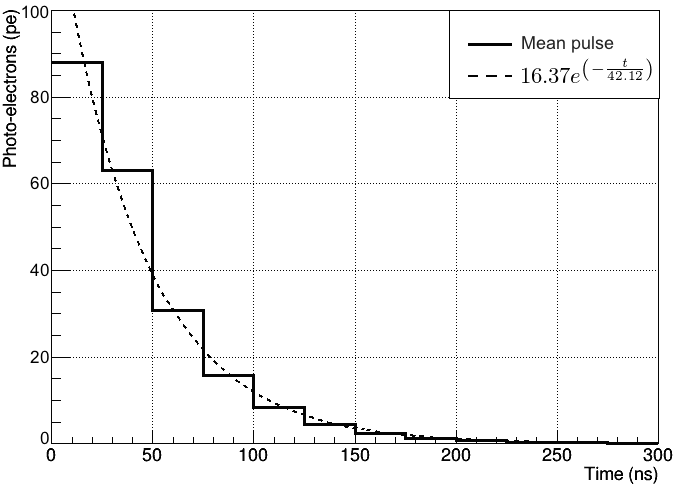
\includegraphics[width=0.45\textwidth]{Figures/pulse_vem.png}
\caption{Number of Cherenkov photons impinging the PMT for 3 GeV muons crossing the WCD. The solid-line represents the average number of photo-electrons and the dashed-line the best exponential fit. The attenuation time is $\sim$ 42.12~ns and the pulse width (at the 10$\%$ amplitude) is $\sim$100~ns \cite{Vasquez2019}}
\label{pulse_G4}
\end{center}
\end{figure}

%The figure shows the number of cherenkov photons $N_{\gamma}$ hitting the PMT surface during a short period of time. In order to calculate the number of photo-electrons $N_{pe}$ generated by photoelectric effect in the PMT cathode is necessary introduce the quantum efficiency Q.E. of the PMT, Fig. \ref{QE}.

% \begin{figure}[h!]
% \begin{center}
% 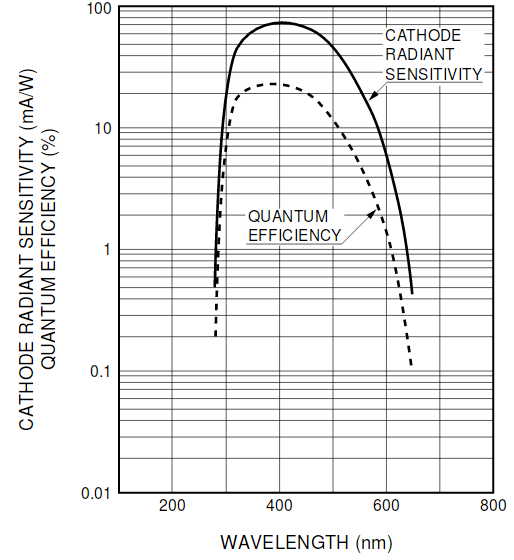
\includegraphics[width=0.4\textwidth]{Figures/QE}
% \caption{Quantum efficiency for the PMT R5912.}
% \label{QE}
% \end{center}
% \end{figure}

The photocathode current $I_k$ is 

\begin{equation}
I_k = \frac{Q}{t}
\end{equation}

\noindent where $Q$ is the electric charge in the photocathode, defined as

\begin{equation}
Q = N_{pe}*e
\end{equation}
with $e$ the electron charge ($1.6 \times 10^{-19}$~C). 

\begin{figure}[h!]
\begin{center}
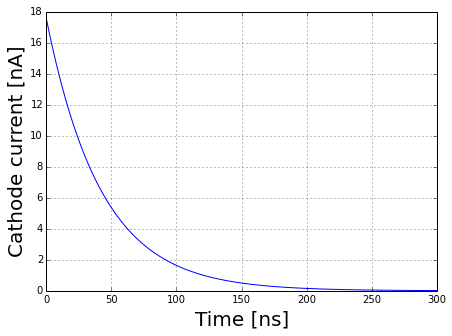
\includegraphics[width=0.45\textwidth]{Figures/Cathode_current}
\caption{Photocathode current taking into account the PMT quantum efficiency ($\eta = 22 \%$) and the number of Cherenkov photons created by 3 GeV muons crossing the WCD.}
\label{cathode}
\end{center}
\end{figure}

In Fig. \ref{cathode} we show the estimated photocathode current for 3 GeV vertical muons impinging the WCD. The maximum peak of the current is $\sim$17 nA which can generate a 17 mA anode current when the PMT gain is 10$^6$. The maximum anode dark current (unwanted current which occurs even in the absence of incident light, resulting from thermally excited electrons ) establishes the low boundary of acquisition 0.7~$\mu$A.

\section{RESULTS}

\subsection{Simulated vertical muon charge}

The PMT model was biased at 1000 V (2.9$\times$10$^5$ gain). When a vertical muon hits the WCD, a current signal of $\sim$5~mA is measured at the anode and a voltage pulse of 250 mV appears across the load resistance (50~$\Omega$). 

The LAGO readout system digitizes the PMT pulses at 40 MHz with a resolution of 10 bits (1 mV/UADC); the pulse shape is stored in a 12 samples vector (300 ns) \cite{SofoHaro2016}. We emulate the digitization process of the model outputs to compare simulations and data. The resulting pulse charge of the simulated vertical muon was 321.6 UADC differing in about 4$\%$ of the value obtained by the MuTe WCD (333 UADC).


% \begin{figure}[h!]
% \begin{center}
% 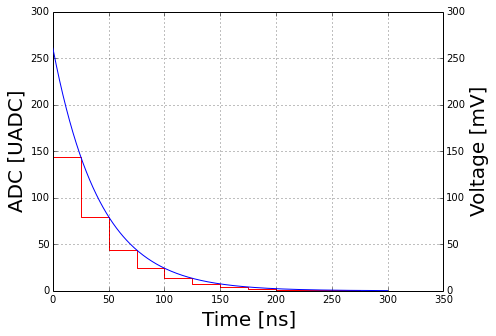
\includegraphics[width=0.5\textwidth]{Figures/dig_pulse.png}
% \caption{Gain curve obtained from the Spice simulation.}
% \label{digitized}
% \end{center}
% \end{figure}

\subsection{Response of the PMT and bias chain model}

Fig. \ref{Pulse} shows the dynode and anode output for a photocathode current of 3.5 nA and a bias voltage of 1000~V. The dynode pulse maximum is 375 mV and the anode is 50 mV. The dynode/anode ratio  is $\sim$7.5 showing that the PMT amplifies 2.66 times the current flowing from the last dynode to the anode. The resulting pulse width $\sim50$~ns occurs by action of the coupling capacitors (C18 and C21).

\begin{figure}[h!]
\begin{center}
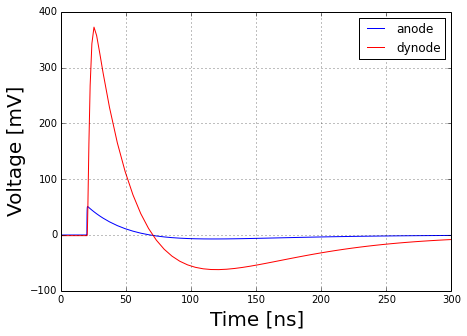
\includegraphics[width=0.48\textwidth]{Figures/spice_pulse.png}
\caption{Anode (blue) and dynode (red) outputs obtained from the Spice model at 1000~V for a cathode current of 3.5~nA. The dynode/anode ratios is 7.5 and the pulse width is $\sim50$~ns.}
\label{Pulse}
\end{center}
\end{figure}

% \begin{figure}[h!]
% \begin{center}
% 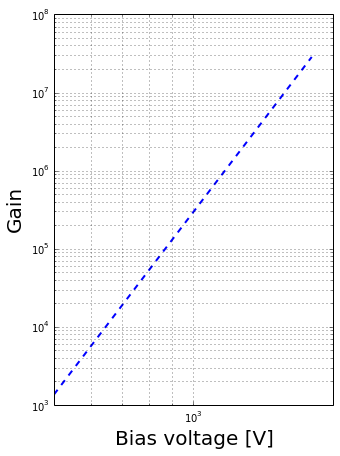
\includegraphics[width=0.35\textwidth]{Figures/Gain_model}
% \caption{Gain curve obtained from the Spice simulation.}
% \label{QE}
% \end{center}
% \end{figure}

%\subsection{Linearity}

The PMT and electronics readout must have a linear behaviour to guarantee an accurate estimation of the deposited energy of particles crossing the WCD. The linearity of the model was estimated correlating the dynode and anode pulse amplitude for different photocathode currents and bias voltages \cite{Arnaldi2019}. Fig. \ref{Linear} correlates the anode and dynode amplitudes for photocathode currents ranging between 0.6-2.2 nA ($V_B$= 1200~V) and 1.3-4.5 nA ($V_B$= 1100~V).

\begin{figure}[h!]
\begin{center}
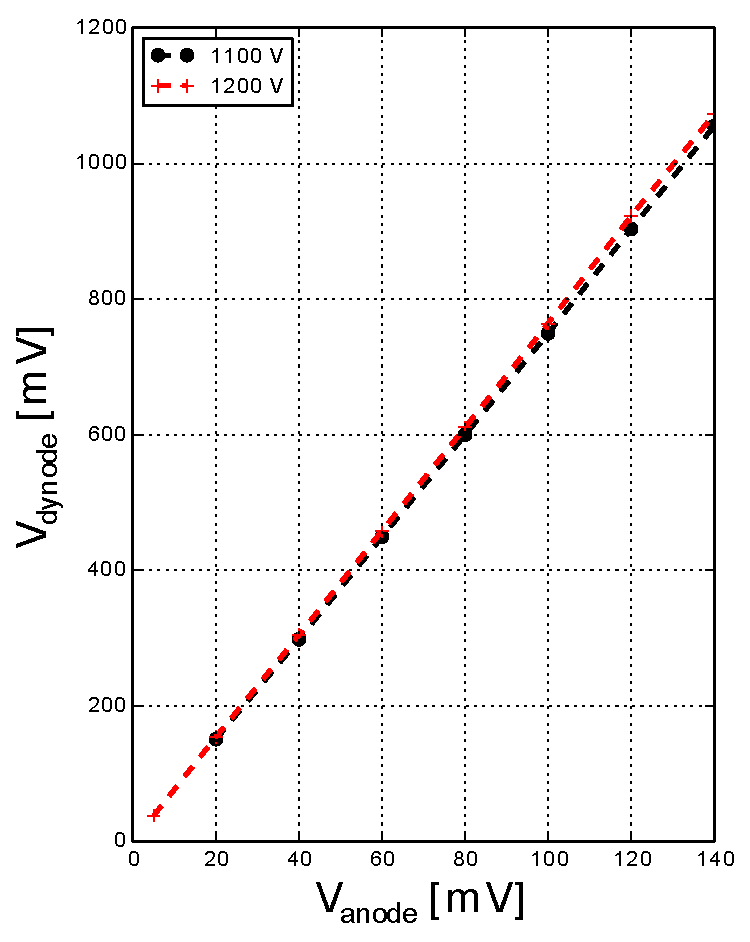
\includegraphics[width=0.4\textwidth]{Figures/Linear.eps}
\caption{Correlation between the dynode and anode output voltage at 1200\,V (red) and 1100\,V (black) for photocathode currents ranging 0.6-4.5 nA.}
\label{Linear}
\end{center}
\end{figure}

The curve slope increases sightly with the bias voltage from 7.52 at 1100~V to 7.68 at 1200~V representing a gain increment of $\sim$2. The linear response of the PMT breaks when the PMT reaches its electrical limits at 1800~V (3$\times10^7$ gain) causing a saturation effect in the pulse amplitude. 

\subsection{Model and data comparison}

\begin{figure}[h!]
\begin{center}
\includegraphics[width=0.45\textwidth]{Figures/Base.eps}
\caption{PCB implementation of the Spice model. The bias voltage is supplied by an EMCO C20 DC/DC converter. The anode and dynode outputs are connected through 50\,$\Omega$ SMA connectors. A DB15 connector inputs the C20 control signal and the conditioning circuit (dynode amplification) supply. The tapered resistance chain was installed in the top layer while the conditioning circuit is in the bottom layer. The anode (P) and the cathode (K) electrodes are highlighted on the figure.}
\label{Base}
\end{center}
\end{figure}

We assess the model performance in two ways: a functional comparison with the present PMT base of LAGO, designed by the Pierre Auger Collaboration (Base-II) \cite{Genolini2001}, and a linearity comparison with data collected by the WCD Chitaga and Nahuelito. 

The PCB (Printed Circuit Board) of the proposed bias circuit (Base-I) is shown in Fig. \ref{Base}. The tapered resistive chain is biased by the EMCO C20 DC/DC converter. The output DC coupling was set by SMD (surface-mount device) capacitors to avoid electrostatic discharges and mechanical damages, as observed in the Base-II. The PCB was electrically isolated with a paint coating with a dielectric strength of 100\,kV/mm.

The first test consisted of comparing the electrode voltage distribution of the Spice model and the Bases I and II. The data was normalized respect to the anode (P) voltage. From Fig. \ref{Comparison} we observe an average variation of 0.7$\%$ between the Base-II and the model while between the Base-II and the Base-I the variation is 2.8$\%$.

\begin{figure}[h!]
\begin{center}
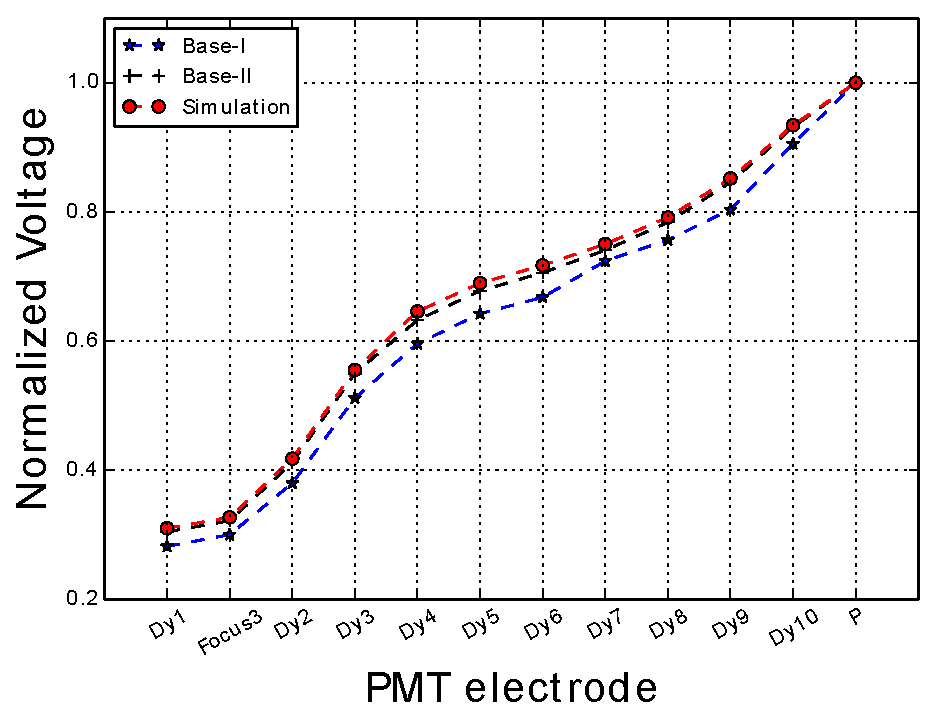
\includegraphics[width=0.48\textwidth]{Figures/LAGO_Auger.eps}
\caption{Comparison of the electrode voltage distribution between the Spice model (red-line), the Base-I (blue-line) and II (black-line).}
\label{Comparison}
\end{center}
\end{figure}

The model was also compared with data of 30$\times 10^3$ pulses recorded by the Nahuelito and Chitaga WCDs as shown in Fig. \ref{Nahuelito_Chitaga}. The Nahuelito's PMT operates at 1500\,V with a discrimination threshold of 70 mV. The WCD data follows a linear distribution with the majority of the recorded events under 100 mV amplitudes. The dashed black-line represents the PMT response obtained from the Spice model.

The Chitaga's PMT operates at 1000~V with a discrimination threshold of 100 mV. The pulse charge distribution is linear but wider than Nahuelito because of the detector geometry differences.

%Another key parameter that changes the data distribution is the water quality of the WCDs.

\begin{figure}[p]
\begin{center}
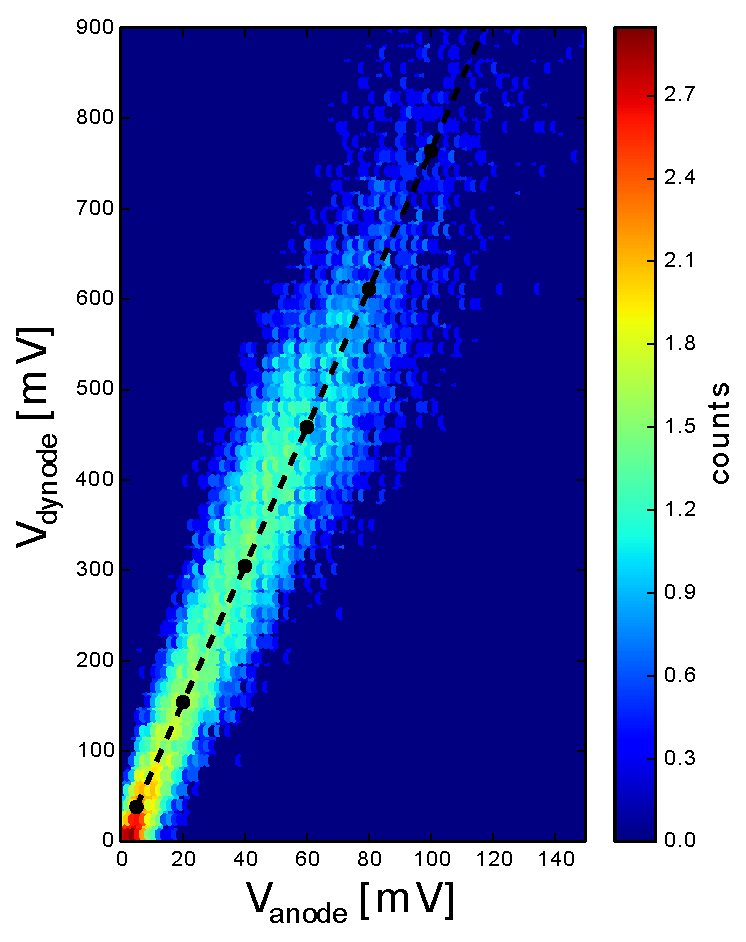
\includegraphics[width=0.4\textwidth]{Figures/Nahuelito.eps}
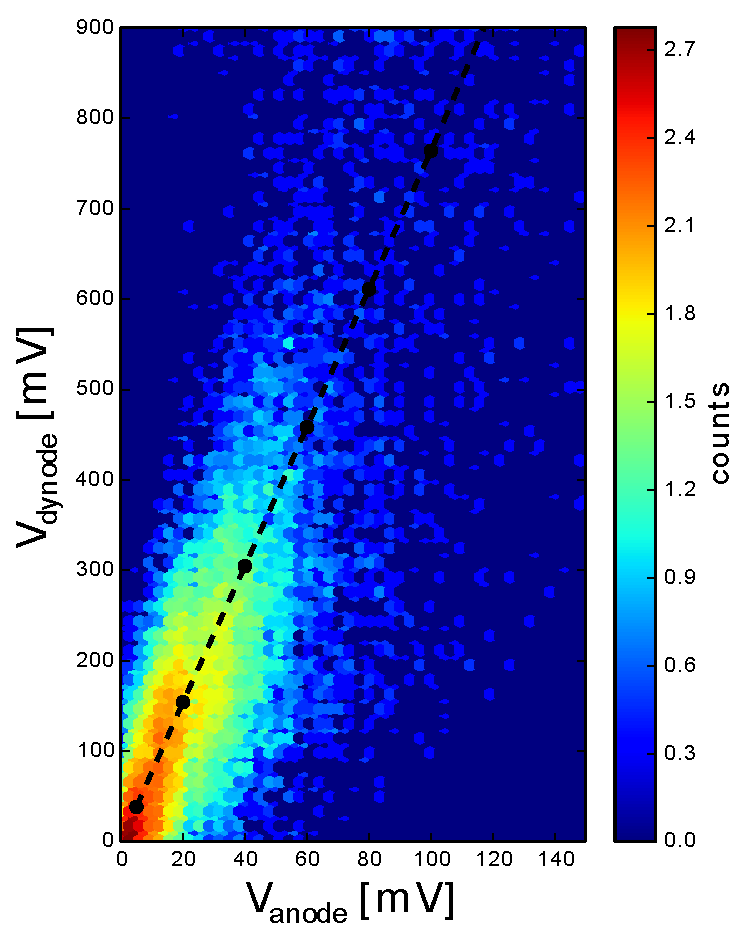
\includegraphics[width=0.4\textwidth]{Figures/Chitaga.eps}
\caption{Linearity measured on the WCDs Nahuelito and Chitaga operating at 1500~V and 1000~V respectively. The data shows the correlation between the maximum amplitude measured on the dynode and the anode with the LAGO's readout electronics. The dashed-line represents the model response taking into account the WCD operation conditions.}
\label{Nahuelito_Chitaga}
\end{center}
\end{figure}

\section{CONCLUSIONS}

A PMT and resistive chain model was designed and tested for the LAGO collaboration. The PMT model reproduces the expected gain depending on the bias voltage as well as the voltage distribution along the dynodes with a variance of $\sim$2.8$\%$. The model can be adapted to any PMT architecture by changing the number of electrodes, the voltage distribution ratio and the parameters $k$ and $\alpha$ -- derived from the PMT datasheet.

The vertical muon charge estimated by the model (321.6 UADC) differs only in 4$\%$ from the measured by the MuTe WCD (333 UADC). The linear correlation between the anode and dynode amplitudes of the model and the data recorded by the WCD Chitaga and Nahuelito were evaluated. 

In this PMT Spice model we set a uniform PMT quantum efficiency of 22$\%$ --the maximum. To obtain more accurate results, we recommend to use the quantum efficiency curve of the modeled PMT where the detection efficiency will change depending on the incident photon wavelength.

\addtolength{\textheight}{-12cm}   % This command serves to balance the column lengths
                                  % on the last page of the document manually. It shortens
                                  % the textheight of the last page by a suitable amount.
                                  % This command does not take effect until the next page
                                  % so it should come on the page before the last. Make
                                  % sure that you do not shorten the textheight too much.

%%%%%%%%%%%%%%%%%%%%%%%%%%%%%%%%%%%%%%%%%%%%%%%%%%%%%%%%%%%%%%%%%%%%%%%%%%%%%%%%


% \section*{APPENDIX}

% Appendixes should appear before the acknowledgment.

\section*{ACKNOWLEDGMENT}

The authors acknowledge  financial support of the Halley Research Group at Universidad Industrial de Santander. We are also very thankful to LAGO and to the Pierre Auger Collaboration for their continuous support.

\bibliographystyle{unsrt}
\bibliography{LAGO.bib}



\end{document}
